% !TEX root = SystemTemplate.tex

\chapter{Overview and concept of operations}

This chapter contains a  general overview of the DanceSoft project. [MB]


\section{Scope}
The scope of this project is to develop a system that allows the academy to manage it's activities and information in an effective manner. Allowing the academy to manage their employees and their students.[MB] 


\section{Purpose}
The purpose of this document is to describe and detail the major components of the system and how
they will be developed. The major components of the application are as follows:

\begin{enumerate}
\item Major System Components
\item System Goals
\item Concept of Operations (CONOPS)
\item System Overview
\item Technologies Used
\end{enumerate} [MB]

\section{Deliverables} 
Listed below are the deliverable major system componets for this project. [MB]

\subsection{Major System Component: Database}
The first major component of the system is the MySQL relational database. The database contains the Academy's data and is the core of the back-end side of the software. This database will be the conduit for most of the systems interactions with the data. The database will live within a local computer provided by the user.  

\subsection{Major System Component: User Interface}
The second major component of the system is the front-end user interface for admins and teachers. This will be the only part of the system most users ever see, and will provide an effective means to complete the desired user task. This is accomplished through the use of pages created in PyQt with interfaces to give users effective ways to interact with the database and the necessary data for their requested operations.

\subsection{Major System Component: Student Interface}
ADD LATER (AFTER WINTER BREAK)

\section{System Access}
Listed below are the various access information, or credentials for the various levels of the system. [MB]

\subsection{Local System GUI}
\subsection{Student Web Interface}
\subsection{Database Access}
ADD LATER (AFTER ACCESS IS FINALIZED IN DEPLOYMENT BOX)

\section{Systems Goals}
The system needs to provide a solution which can run the dance studio data and some day to day activities in an effective and secure manner. This includes allowing teachers to print role sheets, look at schedules, and manage their information. Students need to have the ability to see information pertinent to them such as registration and class requirements. Owners need to be able to use the system to manage their employees, the academy's students and it classes, and other administrative duties such as billing and payroll  Lastly this system as a whole also needs to be an improvement on the current system in use by the customer and provide an easier and more efficient way to run the clients business.

Overall the system goal is to provide a environment where academy owners, teachers, and students can effectively manage their personal needs and requirements for academy participation and continued operations.

\section{Concept of Operations}
This section will cover how the system is used from the viewpoint of the various types of users.

\subsection{New Users}

\subsubsection{New User: Admin}
\subsubsection{New User: Teacher}
UPDATE AS NEW USER PROCESS IS LAID OUT (MOST LIKELY END OF SPRINT 4)
\subsubsection{New User: Student}
UPDATE AS STUDENT INTERFACE IS DESIGNED

\subsection{Existing Users}
This section will cover the options for a user already established in the system.

\subsubsection{Existing User: Admin}

\paragraph{Landing Page}
This page contains the Admin related options

\paragraph{Manage Employees}
This page contains the list of admin functionality associated with the employee functionality

\subparagraph{Search Teachers}
The user is brought to a new window where the user can enter a employees name and see a list of matching teachers. This can also be done using advanced search to search on other fields such as phone number or address. After the search is completed then the user can click on a result to bring up more detailed information and change it as needed. 

\subparagraph{Update Teacher}
The user is prompted with a form where they can select a teacher. After teacher selection the form is populated with that teachers information, the user can then change the information as needed and click the submit button to confirm the changes and submit to the database.

\subparagraph{Assign Teacher To Class}
Opens a window that contains the list of classes ordered alphabetically. The user then selects a class, after class selection the pages generates a list of available teachers by cross referencing their current classes. A teacher is then selected and confirmed before submission to the database. If the selected class is already assigned then a dialog ask the user to confirm the teacher change if yes then the user selects a new teacher and confirms the selection.

\subparagraph{New Teacher}
The user is prompted with an empty form to input teacher information. The user clicks submit when finished and confirms the information before submission to the database.

\paragraph{Manage Classes}
This opens a page containing the list of admin functionality relating to class management.

\subparagraph{View Class}
UPDATE WHEN FUNCTION FINALIZED

\subparagraph{Modify a Class}
The user is prompted with a form where they can select a class. After class selection the form is populated with that classes information, the user can then change the information as needed and click the submit button to confirm the changes and submit to the database.

\subparagraph{Add a Class}
The user is prompted with a form, and asked to fill out the necessary information and click the submit button. This then produces a dialog box to confirm the submission and make the final add to the database.

\paragraph{Manage Students}
This page contains the list of admin functionality associated with the student functionality

\subparagraph{Search Students}
Like the employee search above, the user is brought to a new window where the user can enter a student's name and see a list of matching students. This can also be done using advanced search to search on other fields such as phone number or address. After the search is completed then the user can click on a result to bring up more detailed information and change it as needed. 

\subparagraph{Modify Student Information}
The user is prompted to enter a student name and if the student exist the form is populated and the user can change the information as needed and updates can be submitted to the database.
(FUNCTIONALITY CURRENTLY BEING REEVALUATED MAY MERGE WITH SEARCH FUNCTION)

\subparagraph{Add/Remove Student From Class}
The user is given a list of classes, the user then selects a class. After the class is selected the students currently in the class are displayed. The user can then select a student and click the remove button, or they can click the add button to add a student that has a pending registration to the selected class.

\bf(need user story updates to see if only pending students should show up)


\subparagraph{Registration}
UPDATE AS FUNCTIONALITY IS ADDED


\subsubsection{Existing User: Teacher}

\paragraph{Student Options}
This buttons opens up the the teachers student related functionality.

\subparagraph{Modify Student Info}
When the user selects this option the system will open up a form where a student can be selected and the form will be populated. Then the user can modify the information in the form and submit the updates to the database

\subparagraph{Search Students}
The user is brought to a new window where the user can enter a student's name and see a list of matching students. This can also be done using advanced search to search on other fields such as phone number or address. After the search is completed then the user can click on a result to bring up more detailed information and change it as needed. 

\subparagraph{Add Student to Class}
Much like the Admin function for adding and removing students the teacher will get a window where they can select one of the classes they teach. After that the teacher can select a pending student and add them to the class.
\bf(FUNCTIONALITY MAY CHANGE WITH USER STORY CLARIFICATION)

\subparagraph{See Schedule}
The user will open a window which will show them what classes a selected student is enrolled in on which day.
\bf (MORE INFORMATION AS FUNCTION IS COMPLETED)

\paragraph{Class Options}
This buttons opens up the the teachers class related functionality.

\subparagraph{See Schedule}
The user will open a window which will show them what classes they are teaching on which day.
\bf (MORE INFORMATION AS FUNCTION IS COMPLETED)

\subparagraph{Class Info}
The user can select a class and view the class information.

\subparagraph{Role Sheet}
A window comes up where the user can select one of the classes they are currently teaching and the list of students in the class. The user can then hit a print button which will open up a secondary window where the user can modify the list, import a list from a file, preview the list as a pdf, and print the list.

\paragraph{Personal Options}
This buttons opens up the the teacher functionality relating to personal information.

\subparagraph{Enter Hours}
(WORKED ON IN SPRINT 4

\subparagraph{Modify Information}
(MAY DROP FUNCTIONALITY SINCE IT SHOULD ONLY BE AN ADMIN FEATURE)

\subparagraph{RESET PASSWORD}
User will be prompted to enter and confirm there current password and then if the passwords match the users password then the user will be propted to enter a new password after checking password it is updated in the database.

\subsubsection{Existing User: Student}
UPDATE AS STUDENT INTERFACE PROGRESSES







\section{System Overview and Diagram}
Users will access this application through a local GUI or a web application depending on their position within the system. The GUI will be located in the academy local box, and the student web application will be excess able through any web browser.
When a user makes a connection to the website, the pages and data will be sent to the user. Figure 1 shows an overview of the student interface architecture.
When a local GUI user connects the user will navigate through the vareous pages listed above to the desired functionality. Figure 2 shows a simplistic view of the GUI Architecture.
There are three major components to the project, database, student interface, and admin/teacher interface.  Each section is described in more functional detail above and in \bf section 4 Design and Implementation.
\bf (ADD MORE DETAIL AS SYSTEM FINALIZES) [MB]


\bf(ADD FIGUREs AFTER SYSTEM DESIGN FINALIZATION)
\begin{figure}[tbh]
\begin{center}
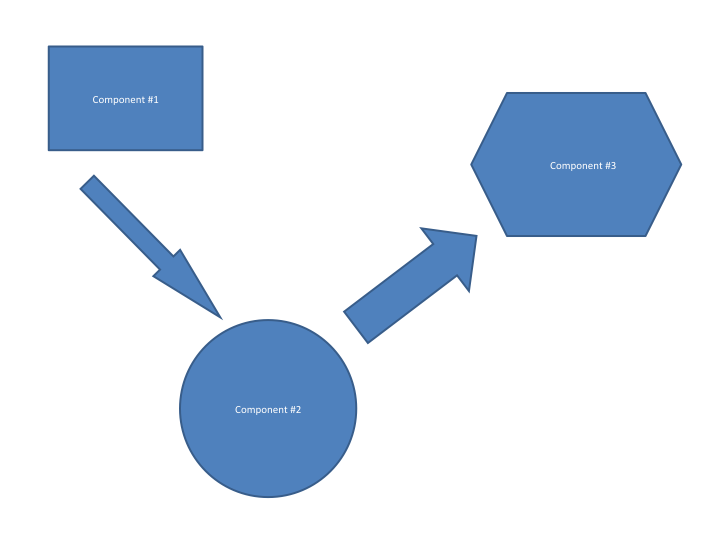
\includegraphics[width=0.75\textwidth]{./diagram}
\end{center}
\caption{A sample figure .... System Diagram \label{systemdiagram}}
\end{figure}

\section{Technologies Overview}
The primary Technologies for this projects are as follows:

\begin{enumerate}
\item Xcode and Visual Studio - Xcode and MSVS are the primary development IDEs for this project. Of the two the one the group used the most was visual studio so we could develop on the machines provided by the school.
\item Python - the primary programming language for the project
\item PHP - primary language for student web interface
\item PyQt and Qt Designer - Gui package and development environment 
\item MySQL - MySQL provides the database and relational quires to manage the data and organize it within the system.
\end{enumerate}


These technologies were selected after a first research sprint where research into programming language, GUI, and database options were selected. A brief description of the research can be found in the sprint 1 report or the first prototype sections of this document. [MB]